% Document setup
\documentclass[12pt]{article}
\usepackage[margin=1in]{geometry}
\usepackage{fancyhdr}
\usepackage{lastpage}

\pagestyle{fancy}
\lhead{Richard Whitehill}
\chead{PHYS 804 -- HW \HWnum}
\rhead{\duedate}
\cfoot{\thepage \hspace{1pt} of \pageref{LastPage}}

% Encoding
\usepackage[utf8]{inputenc}
\usepackage[T1]{fontenc}

% Math/Physics Packages
\usepackage{amsmath}
\usepackage{amssymb}
\usepackage{mathtools}
\usepackage{physics}
\usepackage{siunitx}

\AtBeginDocument{\RenewCommandCopy\qty\SI}

% Enumeration/itemize
\usepackage{enumitem}
\newenvironment{parts}
{\begin{enumerate}[label=\textbf{(\alph*)},leftmargin=*,itemsep=-10pt]
}{\end{enumerate}}

% Reference Style
\usepackage{hyperref}
\hypersetup{
    colorlinks=true,
    linkcolor=blue,
    filecolor=magenta,
    urlcolor=cyan,
    citecolor=green
}

\newcommand{\eref}[1]{Eq.~(\ref{eq:#1})}
\newcommand{\erefs}[2]{Eqs.~(\ref{eq:#1})--(\ref{eq:#2})}

\newcommand{\fref}[1]{Fig.~\ref{fig:#1}}
\newcommand{\frefs}[2]{Figs.~\ref{fig:#1}--\ref{fig:#2}}

\newcommand{\tref}[1]{Table~\ref{tab:#1}}
\newcommand{\trefs}[2]{Tables~\ref{tab:#1}-\ref{tab:#2}}

% Figures and Tables 
\usepackage{graphicx}
\usepackage{float}
\usepackage[font=small,labelfont=bf]{caption}

\newcommand{\bef}{\begin{figure}[h!]\begin{center}}
\newcommand{\eef}{\end{center}\end{figure}}

\newcommand{\bet}{\begin{table}[h!]\begin{center}}
\newcommand{\eet}{\end{center}\end{table}}

% tikz
\usepackage{tikz}
\usetikzlibrary{calc}
\usetikzlibrary{decorations.pathmorphing}
\usetikzlibrary{decorations.markings}
\usetikzlibrary{arrows.meta}
\usetikzlibrary{positioning}
\usetikzlibrary{3d}
\usetikzlibrary{shapes.geometric}

% tcolorbox
\usepackage[most]{tcolorbox}
\usepackage{xcolor}
\usepackage{xifthen}
\usepackage{parskip}

\newcommand*{\eqbox}{\tcboxmath[
    enhanced,
    colback=black!10!white,
    colframe=black,
    sharp corners,
    size=fbox,
    boxsep=8pt,
    boxrule=1pt
]}

% problem-solution macros
% \usepackage{adjustbox}
\usepackage{changepage}

\newtcolorbox{probbox}[1][]{
    breakable,
    enhanced,
    boxrule=0pt,
    frame hidden,
    borderline west={4pt}{0pt}{green!50!black},
    colback=green!5,
    before upper=\textbf{Problem #1) \,},
    % \textbf{Problem #1 \ifthenelse{\isempty{#1}}{}{: #1} \\ },
    sharp corners,
    parbox=false
}

% \newtcolorbox{ProblemBox}[1][]{%
%   breakable,
%   enhanced,
%   colback=black!10!white,
%   colframe=black,
%   title={\large #1 \hfill}
% }
\newcommand{\prob}[2]{
\begin{probbox}[#1]
#2
\end{probbox}
}

\newenvironment{solution}{\begin{adjustwidth}{8pt}{8pt}}{\end{adjustwidth}}
\newcommand{\sol}[1]{
\begin{solution}
#1
\end{solution}
}
% \textbf{#1)} #2}

% Miscellaneous Definitions/Settings
\newcommand{\reals}{\mathbb{R}}
\newcommand{\integers}{\mathbb{Z}}
\newcommand{\naturals}{\mathbb{N}}
\newcommand{\rationals}{\mathbb{Q}}
\newcommand{\complexs}{\mathbb{C}}

\setlength{\parskip}{\baselineskip}
\setlength{\parindent}{0pt}
\setlength{\headheight}{14.49998pt}
\addtolength{\topmargin}{-2.49998pt}


\def\HWnum{Project 1}
\def\duedate{September 25, 2024}

\begin{document}


\section{Introduction}

There are many problems in physics which require minimizing some function with respect to some set of variables.
Of course, many problems in coursework are designed such that the derivatives of the functions of interest can be analytically manipulated to yield a root, or in the worst case, the root can be obtained easily by utilizing graphical methods.
However, practically speaking, most functions are difficult to analytically manipulate in order to yield closed form expressions for the extrema, and when our function depends on a large set of variables, we cannot easily plot the desired function to make direct estimates of the extrema.
That is, to some degree, we are blind to the location of a function's extrema when the dimensionality exceeds our three-dimensional intuition.

In particular, one problem of interest is minimizing the energy of a configuration of particles comprising a molecule.
The potential energy of a configuration of $N$ particles, which we assume here for the sake of simplicity are of the same type, can be modeled through the Lennard-Jones potential
\begin{align}
\label{eq:LJ-N-particle-potential}
    V(\vb*{r}_{1},\ldots,\vb*{r}_{N}) = \frac{4 \epsilon}{2} \sum_{i \ne j} \Bigg( \frac{\sigma^{12}}{|\vb*{r}_{i} - \vb*{r}_{j}|^{12}} - \frac{\sigma^{6}}{|\vb*{r}_{i} - \vb*{r}_{j}|^{6}} \Bigg)
.\end{align}
Note that the factor $1/2$ is inserted to counteract overcounting in the sum, $\epsilon$ is some parameter that determines the strength of the particle interactions, and $\sigma$ is a length scale.
A plot of the potential between two particles is shown in \fref{1d-LJ-potential}.


\begin{figure}[h!tb]
    \centering
    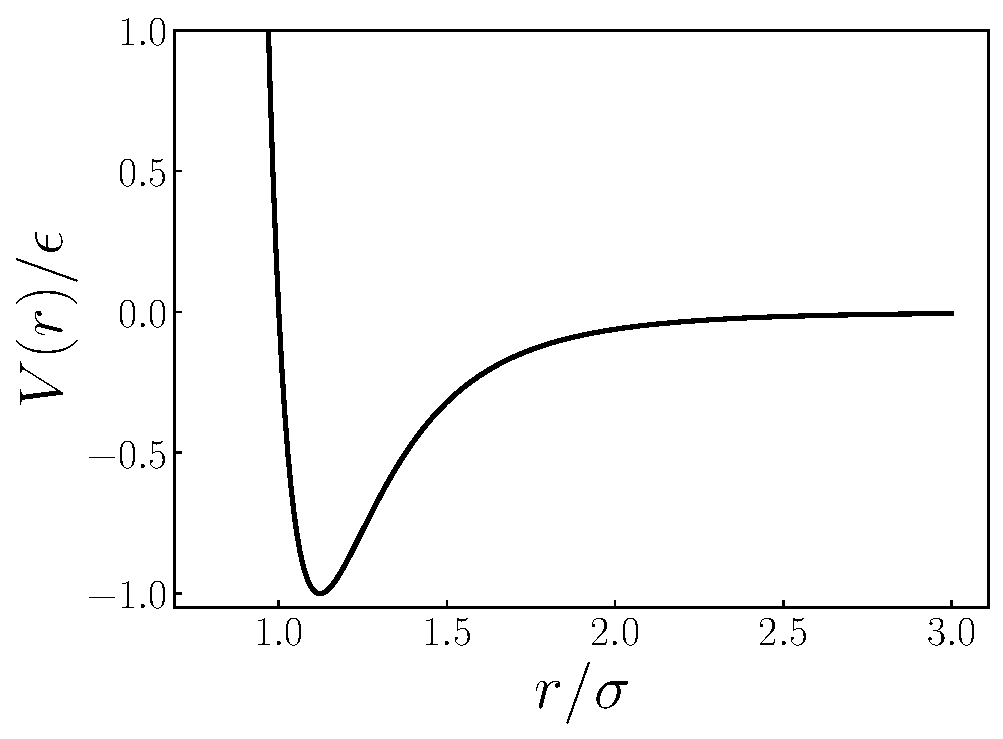
\includegraphics[width=0.5\textwidth]{1d-LJ-potential.pdf}
    \caption{Lennard-Jones potential between two particles as described by \eref{LJ-N-particle-potential}.}
    \label{fig:1d-LJ-potential}
\end{figure}


\section{Framework}

\subsection{Theoretical framework}

For the duration of this work, we redefine our potential and length scales as follows:
\begin{align}
    V \rightarrow V/\epsilon, \quad r \rightarrow r/\sigma
.\end{align}
That is, in the rescaled notation, we have
\begin{align}
    V(\vb*{r}_{1},\ldots,\vb*{r}_{N}) = 2 \sum_{i \ne j} \Bigg( \frac{1}{r^{12}} - \frac{1}{r^{6}} \Bigg)
.\end{align}
such that we only deal with dimensionless quantities in our numerical work.

Before describing the numerical methods we use to find the minima of this potential in the case of $N$-particles, we first explore the analytic solution of this problem.
Certainly, one can solve the problem exactly in the case of two particles.
The potential
\begin{align}
    V(\vb*{r}_1,\vb*{r}_2) = 4 \Bigg( \frac{1}{|\vb*{r}_{1} - \vb*{r}_{2}|^{12}} - \frac{1}{|\vb*{r}_{1} - \vb*{r}_{2}|^{6}} \Bigg)
,\end{align}
and if we transform coordinates such that $\vb*{r} = \vb*{r}_{1} - \vb*{r}_{2}$ and $\vb*{R} = (\vb*{r}_{1} - \vb*{r}_{2})/2$, then
\begin{align}
    V(r) = 4 \Bigg( \frac{1}{r^{12}} - \frac{1}{r^{6}} \Bigg) \Rightarrow V'(r_0) = 4 \Bigg( -\frac{12}{r_0^{13}} + \frac{6}{r_0^{7}} \Bigg) = 0 \Rightarrow r_0 = 2^{1/6}
.\end{align}
We remark on a related set of observations which are interesting from a physics standpoint.
Observe that the result is a single real number.
From the onset, we labeled our potential function as having $4$ degrees of freedom labeled by the $(x,y)$ coordinates of each point.
Indeed, the potential is translationally invariant, meaning that if we take $\vb*{r}_{i} \rightarrow \vb*{r}_{i} + \vb*{a}$, the potential does not change, and this stems from the fact that the interaction between particles is described by a central potential.
Thus, we have eliminated two degrees of freedom.
Additionally, because our potential is central, we can rotate about the $z$-axis, which is perpendicular to the $xy$-plane where our particles live, and the angle of rotation eliminates an additional degree of freedom.

One thing that we have not been careful about above is the following.
In general, we want to minimize the potential with respect to the positions of each particle, implying the condition $\grad_{i} V(\vb*{r}_{1},\ldots,\vb*{r}_{N})$, where $\grad_{i}$ denotes the gradient with respect to $\vb*{r}_{i}$.
Of course, we can translate these conditions in the two particle case under the change of coordinates $\{(x_1,y_1),(x_2,y_2)\}$ to the new coordinates $\{(r,\phi),(R,\Phi)\}$, where $\vb*{r} = r(\cos{\phi} \vu*{x} + \sin{\phi} \vu*{y})$ and $\vb*{R} = R (\cos{\Phi} \vu*{x} + \sin{\Phi} \vu*{y})$ through the chain rule
\begin{align}
\begin{aligned} 
    \pdv{V}{x_1} = \pdv{r}{x_1} \pdv{V}{r} + \pdv{R}{x_1} \pdv{V}{R} + \pdv{\phi}{x_1} \pdv{V}{\phi} + \pdv{\Phi}{x_1} \pdv{V}{\Phi} = 0 \\
    \pdv{V}{y_1} = \pdv{r}{y_1} \pdv{V}{r} + \pdv{R}{y_1} \pdv{V}{R} + \pdv{\phi}{y_1} \pdv{V}{\phi} + \pdv{\Phi}{y_1} \pdv{V}{\Phi} = 0 \\
    \pdv{V}{x_2} = \pdv{r}{x_2} \pdv{V}{r} + \pdv{R}{x_2} \pdv{V}{R} + \pdv{\phi}{x_2} \pdv{V}{\phi} + \pdv{\Phi}{x_2} \pdv{V}{\Phi} = 0 \\
    \pdv{V}{y_2} = \pdv{r}{y_2} \pdv{V}{r} + \pdv{R}{y_2} \pdv{V}{R} + \pdv{\phi}{y_2} \pdv{V}{\phi} + \pdv{\Phi}{y_2} \pdv{V}{\Phi} = 0
.\end{aligned}
\end{align}
Note though that $V$ in the transformed coordinates only depends on $r$, which gives $\pdv*{V}{R} = \pdv*{V}{\phi} = \pdv*{V}{\Phi} = 0$, and therefore, we have transformed our four conditions into a single condition
\begin{align}
    \pdv{V}{r} = 0
\end{align}
as we expected from our symmetry considerations above.

Now, if we move onto the case of three particles, then
\begin{align}
    V(\vb*{r}_{1},\vb*{r}_{2},\vb*{r}_{3}) &= 2 \Bigg[ \Bigg( \frac{1}{|\vb*{r}_{1} - \vb*{r}_{2}|^{12}} - \frac{1}{|\vb*{r}_{1} - \vb*{r}_{2}|^{6}} \Bigg) + \Bigg( \frac{1}{|\vb*{r}_{1} - \vb*{r}_{3}|^{12}} - \frac{1}{|\vb*{r}_{1} - \vb*{r}_{3}|^{6}} \Bigg) \nonumber \\
    &\phantom{2\Bigg[}+ \Bigg( \frac{1}{|\vb*{r}_{2} - \vb*{r}_{3}|^{12}} - \frac{1}{|\vb*{r}_{2} - \vb*{r}_{3}|^{6}} \Bigg) \Bigg]
.\end{align}
Again, we would like to define variables which allows us to retain only the essential degrees of freedom which are uniquely determined at a local minimum of the potential.
One may wish to define relative vectors as in the two-particle case, but these generate a linearly dependent set.
Another natural, albeit less natural, choice of these new coordinates which contains the same number of independent variables is 
\begin{align}
    \vb*{r}_{12} = \vb*{r}_{1} - \vb*{r}_{2}, \quad \vb*{r}_{13} = \vb*{r}_{1} - \vb*{r}_{3}, \quad \vb*{R} = \frac{\vb*{r}_{1} + \vb*{r}_{2} + \vb*{r}_{3}}{3} 
.\end{align}
In these variables, we have
\begin{align}
    V(\vb*{r}_{12},\vb*{r}_{13},\vb*{R}) = 2 \Bigg[ \Bigg( \frac{1}{r_{12}^{12}} - \frac{1}{r_{12}^{6}} \Bigg) + \Bigg( \frac{1}{r_{13}^{12}} - \frac{1}{r_{13}^{6}} \Bigg) + \Bigg( \frac{1}{|\vb*{r}_{12} - \vb*{r}_{13}|^{12}} - \frac{1}{|\vb*{r}_{12} - \vb*{r}_{13}|^{6}} \Bigg) \Bigg]
.\end{align}
Herein, though, lies the primary difficulty of analyzing the many-body problem.
That is, it is difficult (perhaps impossible) to find a set of coordinates which allow us to decouple to essential degrees of freedom in the minimization condition.
Because of time constraints, I have not carried the algebra or calculus any further, but based on the numerical implementation, it may be possible analytically to show that the solution for the three particle configuration is an equilateral triangle.
The procedure introduced here for the three-particle configuration can be generalized to the $N$-particle configuration by introducing the coordinates
\begin{align}
    \vb*{r}_{12} = \vb*{r}_{1} - \vb*{r}_{2}, \quad \ldots, \quad \vb*{r}_{1N} = \vb*{r}_{1} - \vb*{r}_{N}, \quad \vb*{R} = \frac{\vb*{r}_{1} + \ldots + \vb*{r}_{N}}{N}
.\end{align}


\subsection{Code setup and description}
\label{ssec:code-setup-and-description}

In this section because of the analytic complexity and difficulty of solving for the minimum potential for a configuration of particles, in this section, we discuss a numerical Monte Carlo approach, implemented via a random walk, for finding minima of the potential.
Consider an initial configuration $X_0 = \{ \vb*{r}_{1}^{(0)}, \ldots, \vb*{r}_{N}^{(0)} \}$ of the particles on an $L \times L$ square domain, where $L$ is some real number discussed further below.
We can then define a random walk $(X_{n})$ by updating the positions of each particle by the recursive formula
\begin{align}
    \vb*{r}_{i}^{(n)} = \vb*{r}_{i}^{(n-1)} + h ( 2 \vb*{u} - 1 )
,\end{align}
where $h$ is another real-valued hyperparameter and $\vb*{u} \in [0,1]^{2}$ is a uniform random variable.
Thus, the second term implements the random walk by making a step within an $h \times h$ square centered around the previous position.
Note, however, that we only accept the new proposed configuration if $V(X_{n}) < V(X_{n-1})$.
While this procedure can be carried out to any precision, we implement three stopping constraints.
First, we hard-code a maximum number of iterations in the recursion such that if $n > n_{\rm max}$, the most recently accepted configuration is returned.
Next, we implement absolute and relative precision tolerances $\delta_{a}$ and $\delta_{r}$, respectively, such that if
\begin{align}
    |V(X_{n}) - V(X_{n-1})| < \delta_{a} ~ {\rm or} ~ \Bigg| \frac{V(X_{n}) - V(X_{n-1})}{V(X_{n-1})} \Bigg| < \delta_{r}
,\end{align}
the iteration is halted, and $V(X_{n})$ is returned as output.
A \textit{python} implementation of this numerical scheme is displayed in Appendix \ref{app:code-listing}.

\subsection{A brief discussion of hyperparameters}

Note that in the numerical implementation, we are forced to include some non-physical parameters which have an effect on the efficiency, accuracy, and precision of our results, which will be discussed in more detail below.
Here, though, we can describe their assigned values.
In the code below, we choose $L = 2^{1/6} N$ and $h = 0.2$.
We must be careful that our initial $L$ is not too large such that the potential is mostly flat with respect to a given particle's position, which corresponds effectively to a free particle.
On the other hand, if we select too small an $L$, this is less practically problematic, but our particles will eventually diffuse away from each other to a minimum if we choose $h$ well.
Note that if $h$ is chosen too large, the particles will tend to make large jumps in their walk and most new positions will be rejected, but on the other hand, if we choose too small an $h$, our particles will not be able to explore enough of the space to find a global minimum.

While our choice of $L$ is relatively straightforward and only influences the initial configuration directly, the choice of $h$ can be more subtle.
Above, we have only concerned ourselves with finding minima, but our goal is actually more specific: we want to find the lowest energy $N$-particle configuration in the Lennard-Jones potential.
That is, we desire to find a global minimum not just a local one, and while there is only one local minimum for $N = 2$ and perhaps $N = 3$, there are more minima for cases with $N > 4$.
Indeed, with the simple random walk implementation described above, for $N > 4$, we often find local minima which are not the global minimum.

There are a few strategies one can implement to attempt to find a global minimum.
The one implemented here is to run many independent random walks from different starting configurations.
By sampling enough distinct starting positions, we may find more than one local minimum, in which case we select the final configuration resulting in the lowest energy.
Of course, we may still have the issue that this minimum is not a global minimum, but it is less likely and biased than minimizing on only a single configuration.
Additionally, while not done here, this approach is quite amenable to parallelization, which would increase the efficiency of identifying a global minimum and is only then limited by the available hardware given that a single random walk runs fairly quickly.
Another method is aimed at escaping local minima.
When the walk converges on a local minimum, we can increase the value of $h$ significantly, resulting in an effectively new starting configuration and repeat the random walk process until a local minimum is found.
Such a process can be repeated as many times as desired, keeping the configuration corresponding to the lowest energy.


\section{Results}

With all the theoretical and computational preliminaries dealt with, we can produce some plots.
Note that the code implements two approaches.
The first method, coined ``method 1'', minimizes the potential with respect to each particle separately.
That is, we first freeze $\vb*{r}_{2}, \ldots, \vb*{r}_{N}$ and vary $\vb*{r}_{1}$ until a stopping condition is met.
Then, we freeze $\vb*{r}_{1}$ and unfreeze $\vb*{r}_{2}$, varying the latter to minimize the potential.
This process is repeated until we have utilized each particle.
The second method, coined ``method 2'', allows the particles to vary in the random walk simultaneously as described in Section \ref{ssec:code-setup-and-description}.

\frefs{track-min3}{track-min3} demonstrate the results over a single walk for methods 1 and 2 from the same starting configuration on $N = 2$ and $N = 3$.
The programs run quite quickly for each of these setups, and it is observed generally that less iterations are required for method 2 to find a minimum.

\begin{figure}[h!tb]
    \centering
    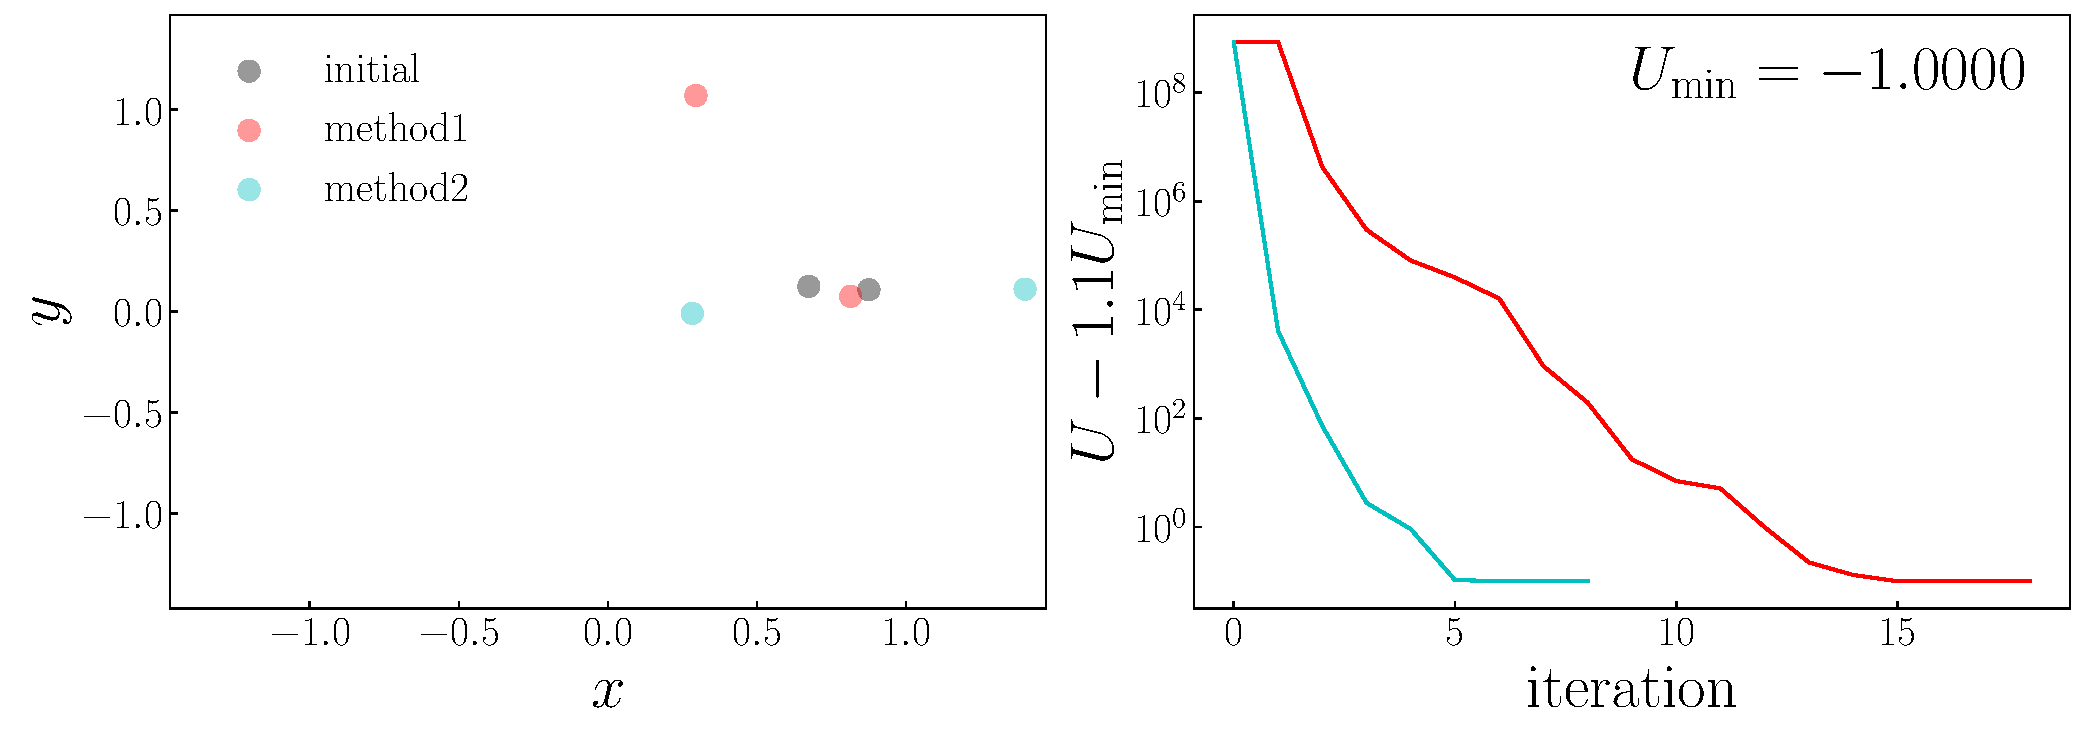
\includegraphics[width=0.8\textwidth]{track_min2.pdf}
    \caption{Results of random walk minimization for $N = 2$.}
    \label{fig:track-min2}
\end{figure}

\begin{figure}[h!tb]
    \centering
    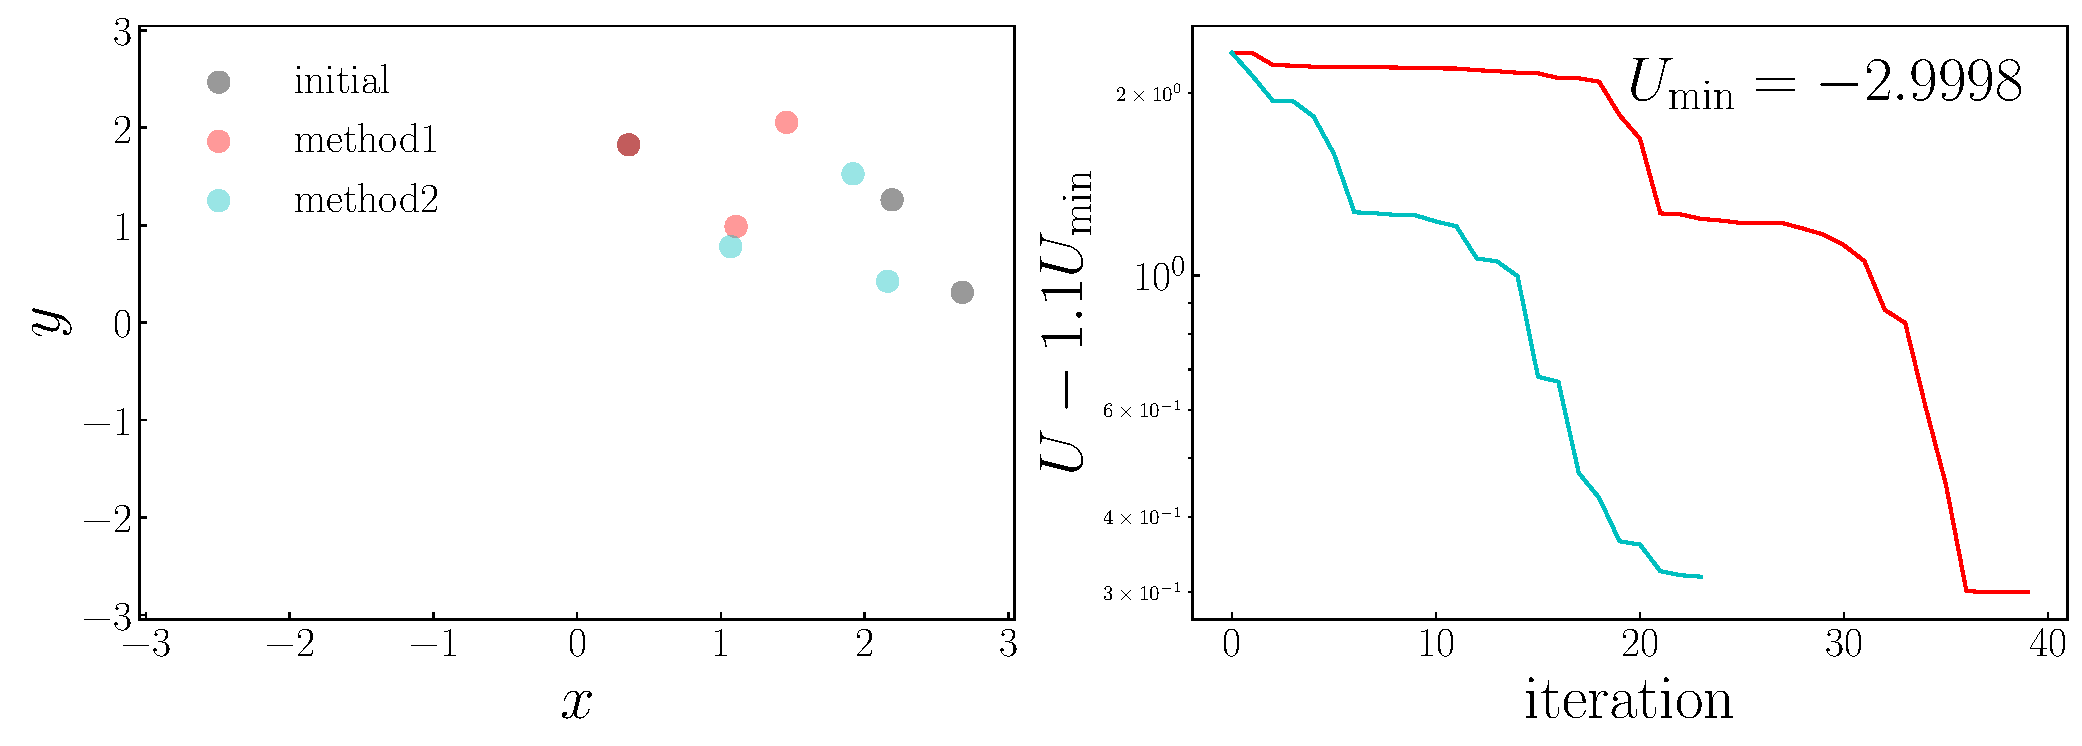
\includegraphics[width=0.8\textwidth]{track_min3.pdf}
    \caption{Results of random walk minimization for $N =3$.}
    \label{fig:track-min3}
\end{figure}

Next, we run the simulation for $N = 4$ as shown in \fref{track-min4} and \fref{track-min10}.
In these cases, we already run into the issue of finding local minima.

\begin{figure}[h!tb]
    \centering
    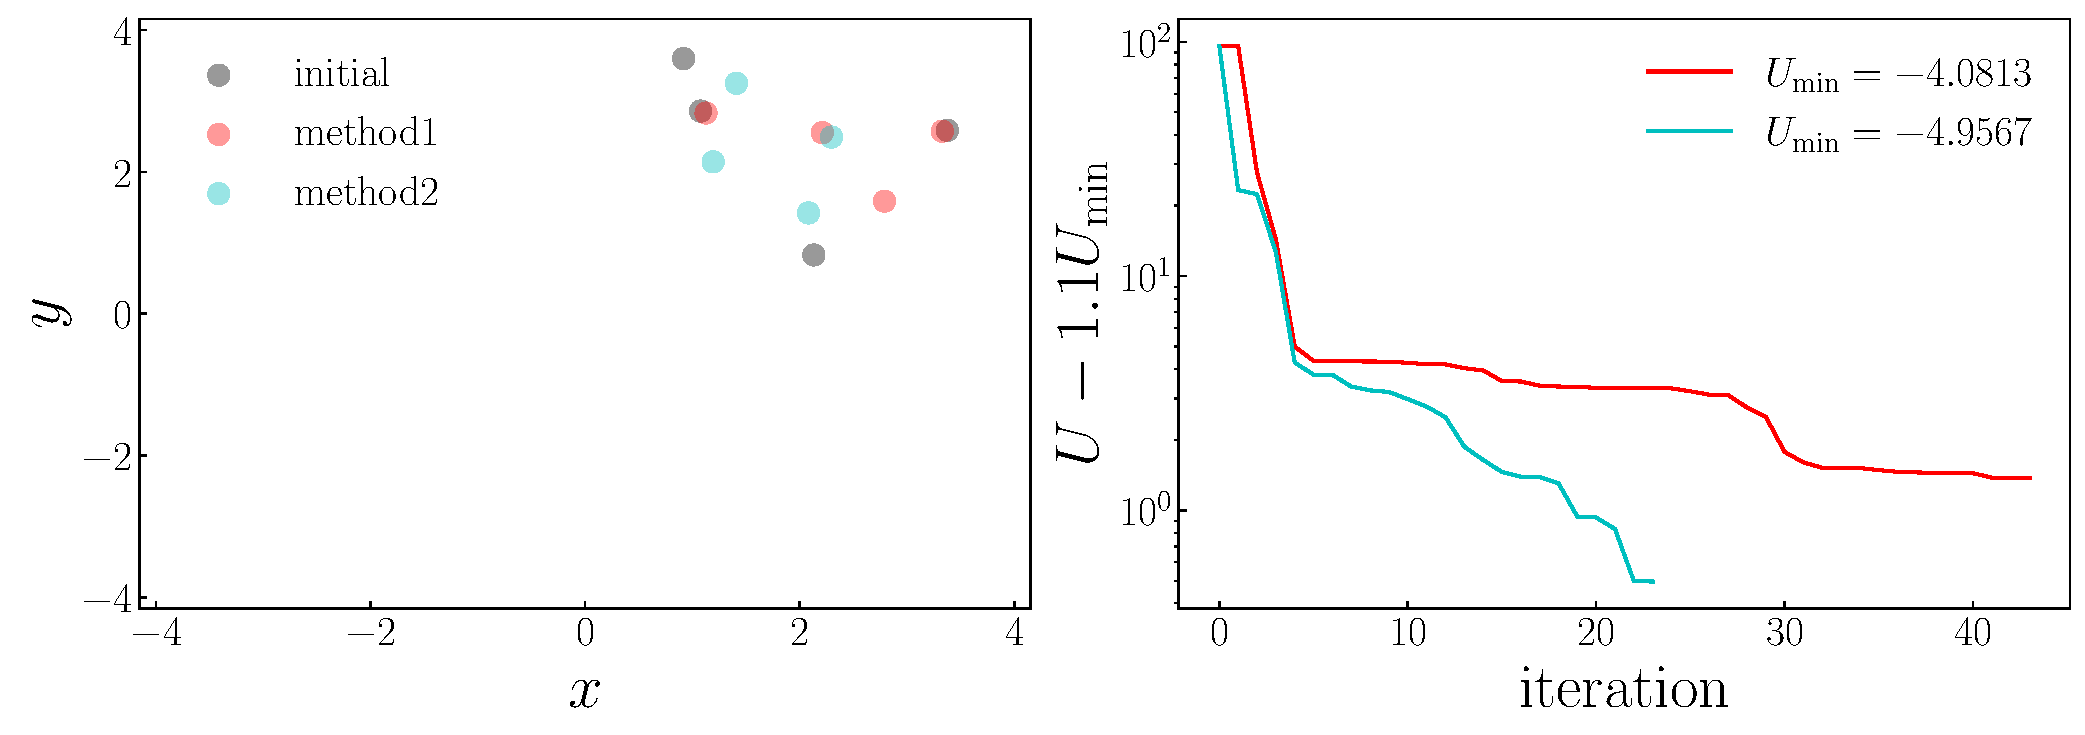
\includegraphics[width=0.8\textwidth]{track_min4.pdf}
    \caption{Results of random walk minimization for $N =4$.}
    \label{fig:track-min4}
\end{figure}

\begin{figure}[h!tb]
    \centering
    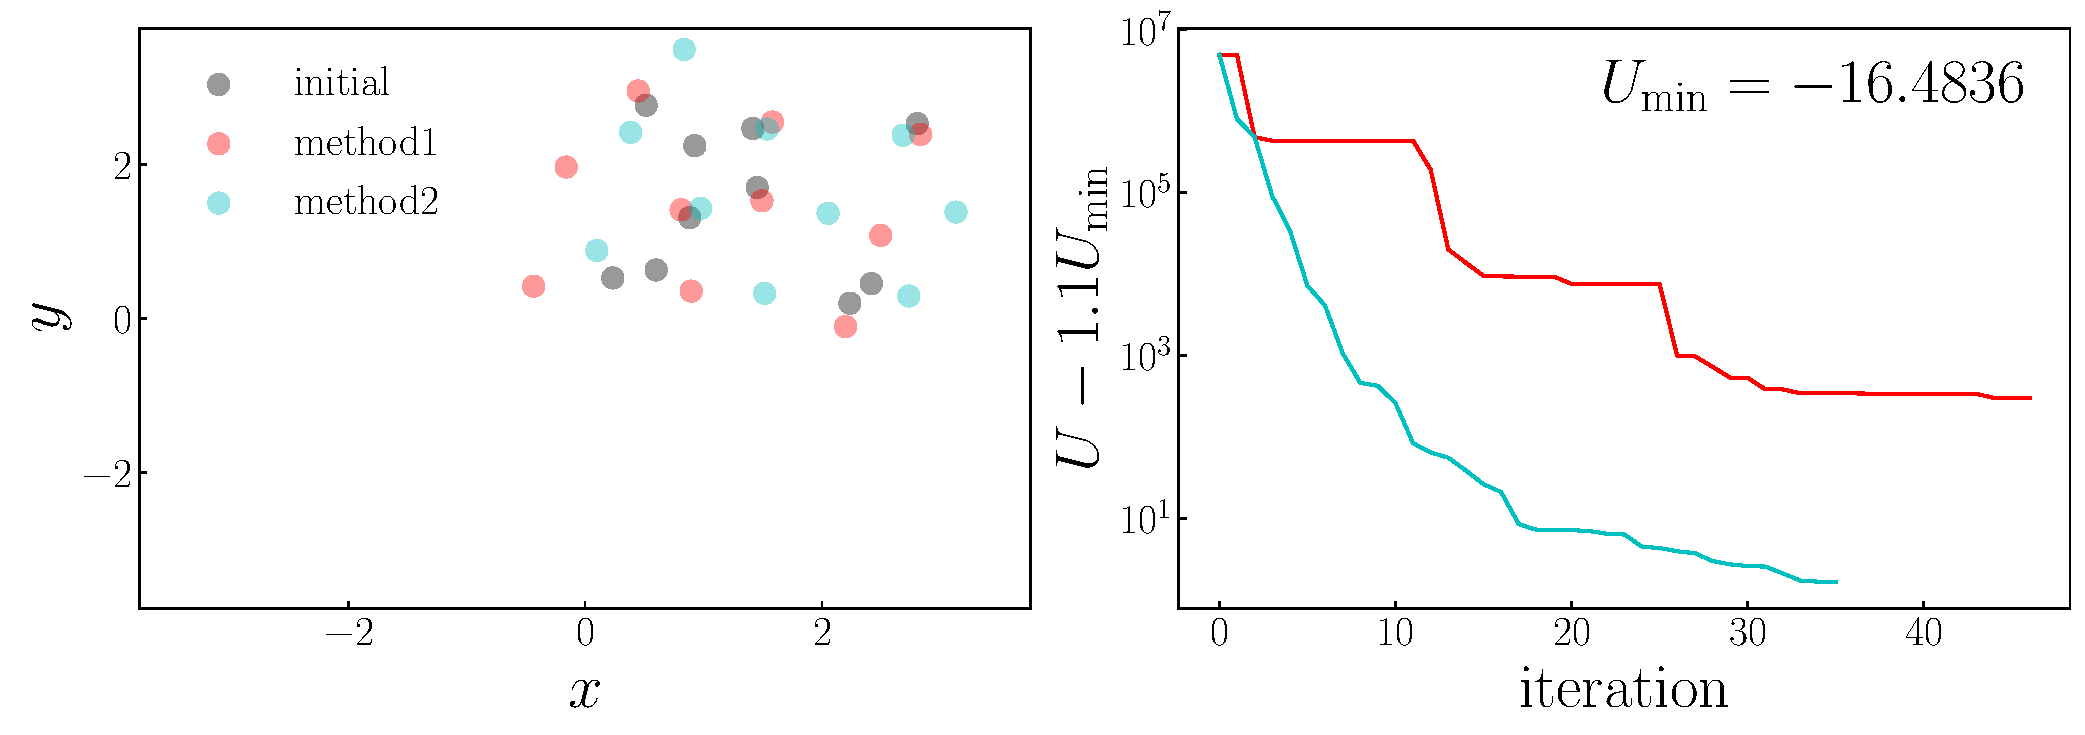
\includegraphics[width=0.8\textwidth]{track_min10.pdf}
    \caption{Results of random walk minimization for $N = 10$.}
    \label{fig:track-min10}
\end{figure}

In \fref{batch-min4}, we display the results of running a batch of minimizations, and as desired, we are able to separate the global minimum from the ensemble of local minima.
Note, though, that the current implementation in a for loop is a very crude and inefficient one.
To generate \fref{batch-min4}, we sampled 100 different initial configurations, and it took nearly 20 minutes on my Mac laptop to minimize all the configurations, although, on average takes less than a minute per configuration to minimize.
As discussed above, this approach should ideally be parallelized to increase efficiency.

\begin{figure}[h!tb]
    \centering
    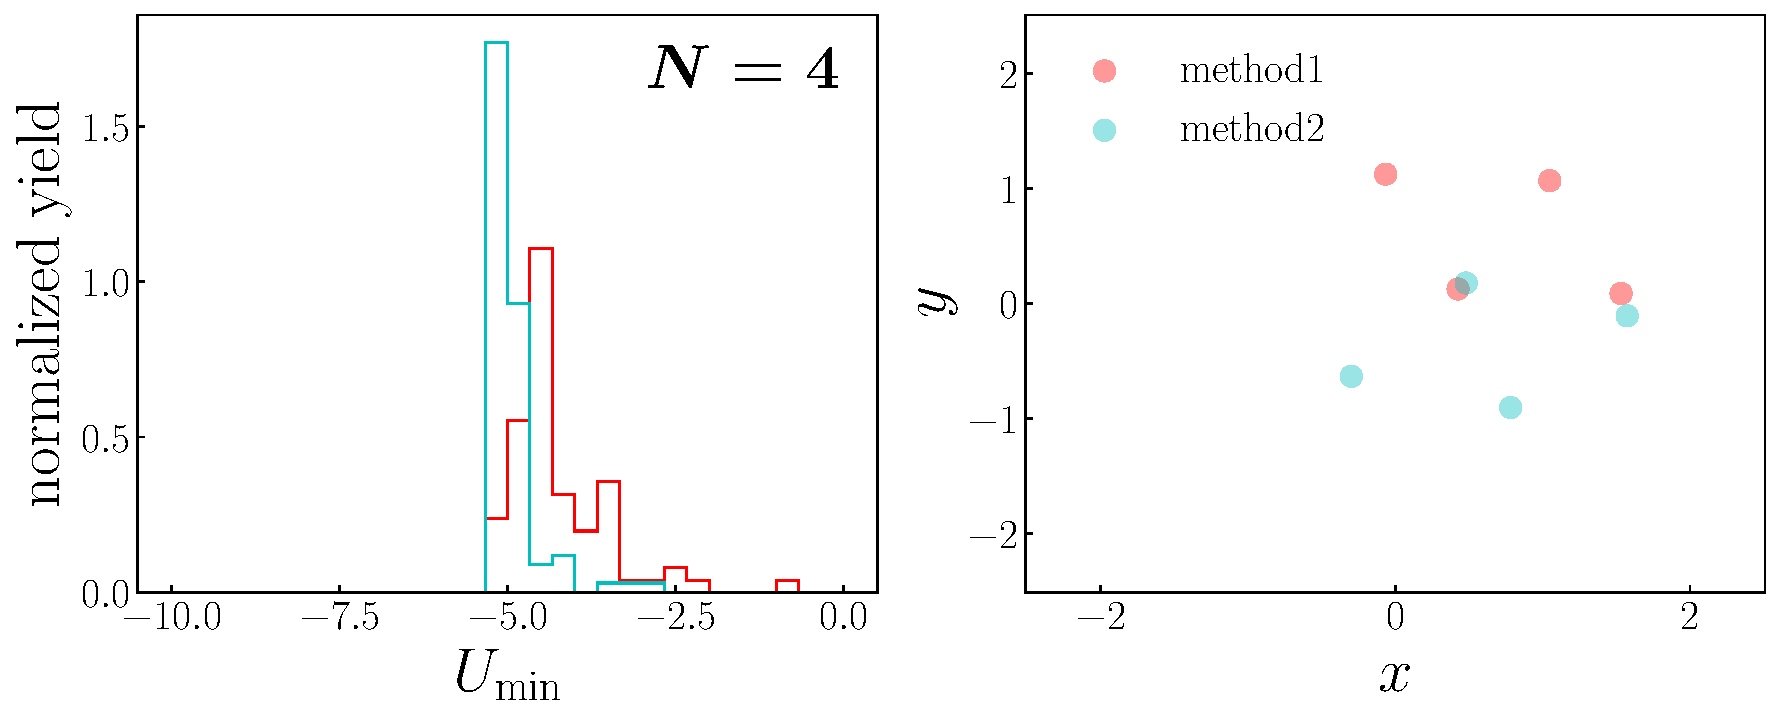
\includegraphics[width=0.8\textwidth]{batch_min4.pdf}
    \caption{Results of a batch random walk minimization for $N = 4$.}
    \label{fig:batch-min4}
\end{figure}


\section{Conclusion}

In this article, we have described the minimization of the Lennard-Jones potential for a system of $N$-particles, analytically and numerically via a random walk Monte Carlo procedure.
While the implementation of the numerical scheme is somewhat crude, we have discussed a few possible adjustments to increase its efficiency.
Alternatively, one could also implement other methods to minimize the potential.
Within the class of Monte Carlo methods, we could utilize some importance sampling or Markov chain method, which would sample the potential and allow us to explore the configuration space in a different way.
There are also minimization procedures that are not based on Monte Carlo methods such gradient descent.
Such methods require more knowledge of the function being minimized or additional numerical schemes to be implemented, but may be better suited for this problem.
Whichever scheme is implemented, there are associated unique issues, but the issue of becoming stuck in local minima is a ubiquitous one, requiring careful consideration in a more serious research setting.

\appendix

\section{Code Listing}
\label{app:code-listing}

\textbf{Main python script}
\inputpython{main.py}

\textbf{Script for single configuration minimization}
\inputpython{single.py}

\textbf{Script for batch configuration minimization}
\inputpython{batch.py}

    
\end{document}
